\section{Marco Metodológico y Estrategias de Refactorización}

Esta sección es nuestro manual de instrucciones. Aquí vamos a contar de forma clara y sencilla el mapa de ruta que seguimos para construir el Portal Agro-comercial del Huila, poniendo siempre el foco en dos cosas: que la calidad fuera incuestionable y que la plataforma funcionara justo como se esperaba.

\subsection{Gestión del Proyecto: La Disciplina de Scrum}

Para que el proyecto avanzara de forma transparente y pudiera adaptarse rápidamente a los cambios o peticiones, elegimos la metodología Scrum.

\paragraph{Ciclo de Trabajo y la Regla del "Terminado"}

\paragraph{Trabajo por Ciclos Cortos:} Definimos periodos de trabajo de dos semanas (llamados Sprints). Gracias a esto, nos obligamos a priorizar y a enfocarnos. Por ejemplo, el Flujo de Pedido (RF-004), que es complejo, lo abordamos en pedacitos durante varios ciclos para no saturar al equipo.

\paragraph{Control Visual con Trello:} Usamos Trello para que todos vieran exactamente en qué estábamos. Pero, además, pusimos un límite a las tareas que podíamos tener a medias (WIP o Trabajo en Progreso). Esto es crucial porque evita que el equipo de C\# empiece algo nuevo si lo anterior no está totalmente finalizado.

\paragraph{Definición de Terminado (Regla de Oro):} Para que una funcionalidad se diera por "Terminada", tenía que pasar filtros muy estrictos:

\begin{itemize}
\item El código debía estar funcionando bien y revisado por otro compañero (Peer Review).

\item Teníamos que tener pruebas automáticas que cubrieran más del 85\% del código nuevo.

\item Y lo más importante, el cambio no podía agregar nueva deuda técnica (código mal hecho o confuso).
\end{itemize}

\paragraph{El Rigor de la Revisión y las Pruebas de Aceptación:}

Para asegurar que el código cumpliera con lo que se necesitaba desde el primer momento, implementamos un proceso riguroso de Revisión de Código y Pruebas de Aceptación. Cada vez que un desarrollador terminaba una parte, otro compañero debía revisarlo a fondo antes de que ese código entrara al proyecto principal. Esto servía para asegurar que los principios de diseño (SOLID) se hubieran aplicado bien, que la lógica fuera fácil de entender y que no hubiera errores evidentes o código confuso.

\paragraph{Pruebas de Aceptación (El Primer Filtro):} Para funcionalidades cruciales, como el Flujo de Pedido (RF-004) o el Login (RF-001), el equipo se enfocó en crear Pruebas de Aceptación que validaban el proceso completo del usuario. Así, estas pruebas automáticas comprobaban, por ejemplo, que si un usuario se registraba, el sistema lo guardara bien y le diera acceso. De este modo, nos aseguramos de que la función más importante fuera correcta y confiable antes de llevarla al control de calidad.

\paragraph{Las 5 Etapas de Construcción del Portal}

El desarrollo se organizó en etapas que se iban completando de forma progresiva, lo que ayudó mucho a reducir el riesgo de que todo fallara al final del proyecto:

\begin{itemize}
\item \textbf{Etapa 1: Planificación:} Primero definimos qué era necesario, dibujamos los diagramas de la base de datos (MER) y elegimos la estructura interna del código para garantizar que las distintas partes trabajaran de forma independiente.

\item \textbf{Etapa 2: Cimientos:} Luego, creamos la base de datos, el sistema de acceso (RF-001) y la estructura base del sistema principal (el backend hecho en C\# ASP.NET Core), aplicando las reglas de diseño iniciales.

\item \textbf{Fase 3: Desarrollo Funcional:} En este momento, metimos la lógica central: Gestión de Fincas/Productos y el Flujo de Pedidos (RF-004), donde las pruebas de aceptación fueron más intensas.

\item \textbf{Fase 4: Pruebas y Ajustes:} Después, nos enfocamos en la velocidad de respuesta (RNF-003) y corregir fallos.

\item \textbf{Fase 5: Implementación Final:} Y por último, se hizo el despliegue en la nube (Azure) para la salida a producción.
\end{itemize}

\subsection{Estructura Arquitectónica: Evitando el Caos}

Para que el software fuera limpio y se pudiera adaptar fácil, lo dividimos en partes muy bien separadas, aprovechando la estructura de C\# ASP.NET Core.

\paragraph{Inversión de Dependencias (DI):} Usamos esta técnica (que es nativa de ASP.NET Core) para establecer una regla simple: la parte más importante del negocio (el servicio que maneja el pedido) no debe hablar directamente con la base de datos. En su lugar, tiene que llamar a un contrato (Interface). Esto es fundamental, porque si decidimos cambiar de SQL Server a otra base de datos, la lógica importante no se ve afectada.

\paragraph{La Abstracción del Patrón Repositorio:}

Justo para evitar que la lógica de negocio dependiera de SQL Server, introdujimos un patrón llamado Repositorio. Piensa en el Repositorio como un intermediario o traductor entre la capa de negocio y la base de datos.

De esta manera, el ProductoService (que es la lógica de negocio) simplemente le pide datos al repositorio. El servicio no tiene idea si el dato viene de una base de datos relacional como SQL Server o de un archivo. Esta separación fue clave para que el código no se enredara y nos da la flexibilidad de usar diferentes tipos de bases de datos para distintas necesidades (esto se llama Persistencia Políglota Preparada). Por consiguiente, estábamos listos para, por ejemplo, mover la gestión del Chat de Pedidos (RF-009) a una base de datos NoSQL más eficiente sin tener que reescribir toda la lógica central de los pedidos.

\paragraph{API Gateway como Traductor:} El sistema que ve el usuario (Angular) solo tiene que hablar con un único punto de entrada conocido. Esto nos sirvió para centralizar la seguridad (RF-001) en ese punto y para gestionar las diferentes versiones del sistema sin afectar a los usuarios.

\subsection{Calidad Continua con DevSecOps}

La clave es que la calidad y la seguridad se incluyeron de forma automática en el proceso de trabajo (DevSecOps).

\paragraph{El Guardián del Código: GitHub Actions}

El proceso automático en GitHub Actions (nuestro sistema de entrega automatizada) actuó como un portero con reglas muy estrictas:

\paragraph{Pruebas Obligatorias:} En primer lugar, cuando se subía código, todas las pruebas automáticas se ejecutaban.

\paragraph{Reglas de Limpieza y Seguridad:} Luego, el sistema revisaba cómo estaba el código:

\begin{itemize}
\item \textbf{Revisión de Seguridad:} Escaneaba el código C\# buscando posibles fallos. Un error, por ejemplo, en la seguridad de acceso o en la base de datos, detenía el proceso.

\item \textbf{Medición de Complejidad:} Comprobaba si el código nuevo era demasiado complicado (Complejidad Ciclomática). Si lo era, el sistema lo marcaba como Deuda Técnica y bloqueaba la entrega.

\item \textbf{Control de Versiones:} Aparte de esto, nos aseguramos de que todos los paquetes y herramientas usadas estuvieran actualizadas y sin problemas de seguridad conocidos, revisando todo con escáneres automáticos.
\end{itemize}

\paragraph{Entrega Segura:} Solo si el código pasaba todos los filtros (era funcional, seguro y limpio), se autorizaba a pasarlo al ambiente de pruebas.

\paragraph{Análisis Automático y Aplicación de Reglas de Higiene de Código:}

Nuestro objetivo no era solo que el código funcionara, sino que fuera limpio y fácil de entender para cualquiera del equipo. Por eso, el sistema de automatización se configuró para aplicar reglas de limpieza estrictas que definimos al inicio del proyecto.

\paragraph{El Termómetro del Código (Complejidad):} Otra regla de higiene vital fue el control de la Complejidad Ciclomática. Esta es una herramienta que nos dice cuántos caminos diferentes tiene una función. Si una función en C\# superaba el número 12 (lo que indica que tiene demasiados si o o anidados), el sistema la identificaba como Deuda Técnica inaceptable y detenía la integración. De este modo, garantizamos que el código no solo hiciera lo que debía, sino que también fuera legible y fácil de mantener.

\paragraph{Inspecciones de Patrones:} Finalmente, el análisis automático comprobaba que el código siguiera los patrones de diseño que habíamos acordado (como el Patrón Repositorio) y avisaba de inmediato si alguien intentaba saltarse la regla de Inversión de Dependencias.

\paragraph{Estrategias de Flexibilidad para el Futuro}

\paragraph{Diseño Anti-Monolito:} A pesar de que el Portal es nuevo, lo construimos pensando en el largo plazo. Por ejemplo, si el Chat de Pedidos (RF-009) crece muchísimo, simplemente podemos separar ese código para que funcione como un servicio pequeño e independiente.

\paragraph{Estar listos para Bases de Datos Mixtas:} Gracias a la separación que logramos con el Patrón Repositorio, si la funcionalidad del Chat necesita una base de datos más rápida y versátil, simplemente podemos cambiar esa parte sin necesidad de reescribir toda la lógica principal de los pedidos.

\subsection{Mantenimiento y Rendimiento: Metas Clave}

La rigurosidad de la metodología tiene un objetivo claro: hacer más fácil y barato el mantenimiento futuro. Por eso, usamos indicadores clave (KPIs) para medir si estamos siendo exitosos:

\paragraph{Tiempo de Corrección (MTTR):} Medimos cuánto tiempo tardamos en arreglar un fallo y devolver el sistema a la normalidad. La meta era poder hacerlo en menos de 60 minutos, un objetivo ambicioso que solo consiguen los equipos de desarrollo más rápidos.

\paragraph{Mantenimiento Evolutivo:} Esto lo medimos con la Frecuencia de Entrega (es decir, cada cuánto podemos lanzar cosas nuevas). Como el código está limpio, podemos liberar mejoras (como el Chat (RF-009) o los QR (RF-012)) a los ambientes de prueba todas las semanas.

\paragraph{Mantenimiento Preventivo:} El trabajo más valioso: mantener la Deuda Técnica en Cero para evitar problemas y gastos innecesarios en el futuro.

\paragraph{La Velocidad de Entrega (Lead Time):}

Para nosotros, ser rápidos significaba ser eficientes. Medimos un factor crucial llamado Lead Time, que es el tiempo total que pasa desde que un desarrollador escribe una línea de código hasta que esa misma línea está funcionando en producción. Con nuestro sistema automatizado, logramos reducir este tiempo de días a solo unas pocas horas, lo que quiere decir que cualquier mejora llega al usuario final de forma increíblemente rápida.

\paragraph{Mitigación de Riesgos y Documentación}

Para el riesgo de lentitud (RNF-003): Hicimos pruebas de rendimiento constantes, simulando muchos usuarios haciendo pedidos. Esto nos obligó a optimizar las consultas en SQL Server y a usar memoria caché en C\# para que la plataforma fuera rápida.

La Resistencia del Equipo: La mejor estrategia fue demostrar con hechos: al usar Pruebas de Aceptación y DevSecOps, había menos fallos, lo que se traducía en menos estrés y menos horas extra no planeadas para el equipo. Además, la documentación técnica que estamos generando sirve como la memoria oficial del proyecto para que el conocimiento no se pierda.

El Clima del Equipo: Y finalmente, medimos algo que no es técnico: la satisfacción del equipo. Un equipo satisfecho y con herramientas que funcionan bien (como el CI/CD) es un equipo que produce código de mejor calidad y que quiere quedarse en el proyecto. Por eso, la documentación y las prácticas no son solo para el software, sino para la gente que lo construye.

\begin{figure}[htbp]
    \centering
    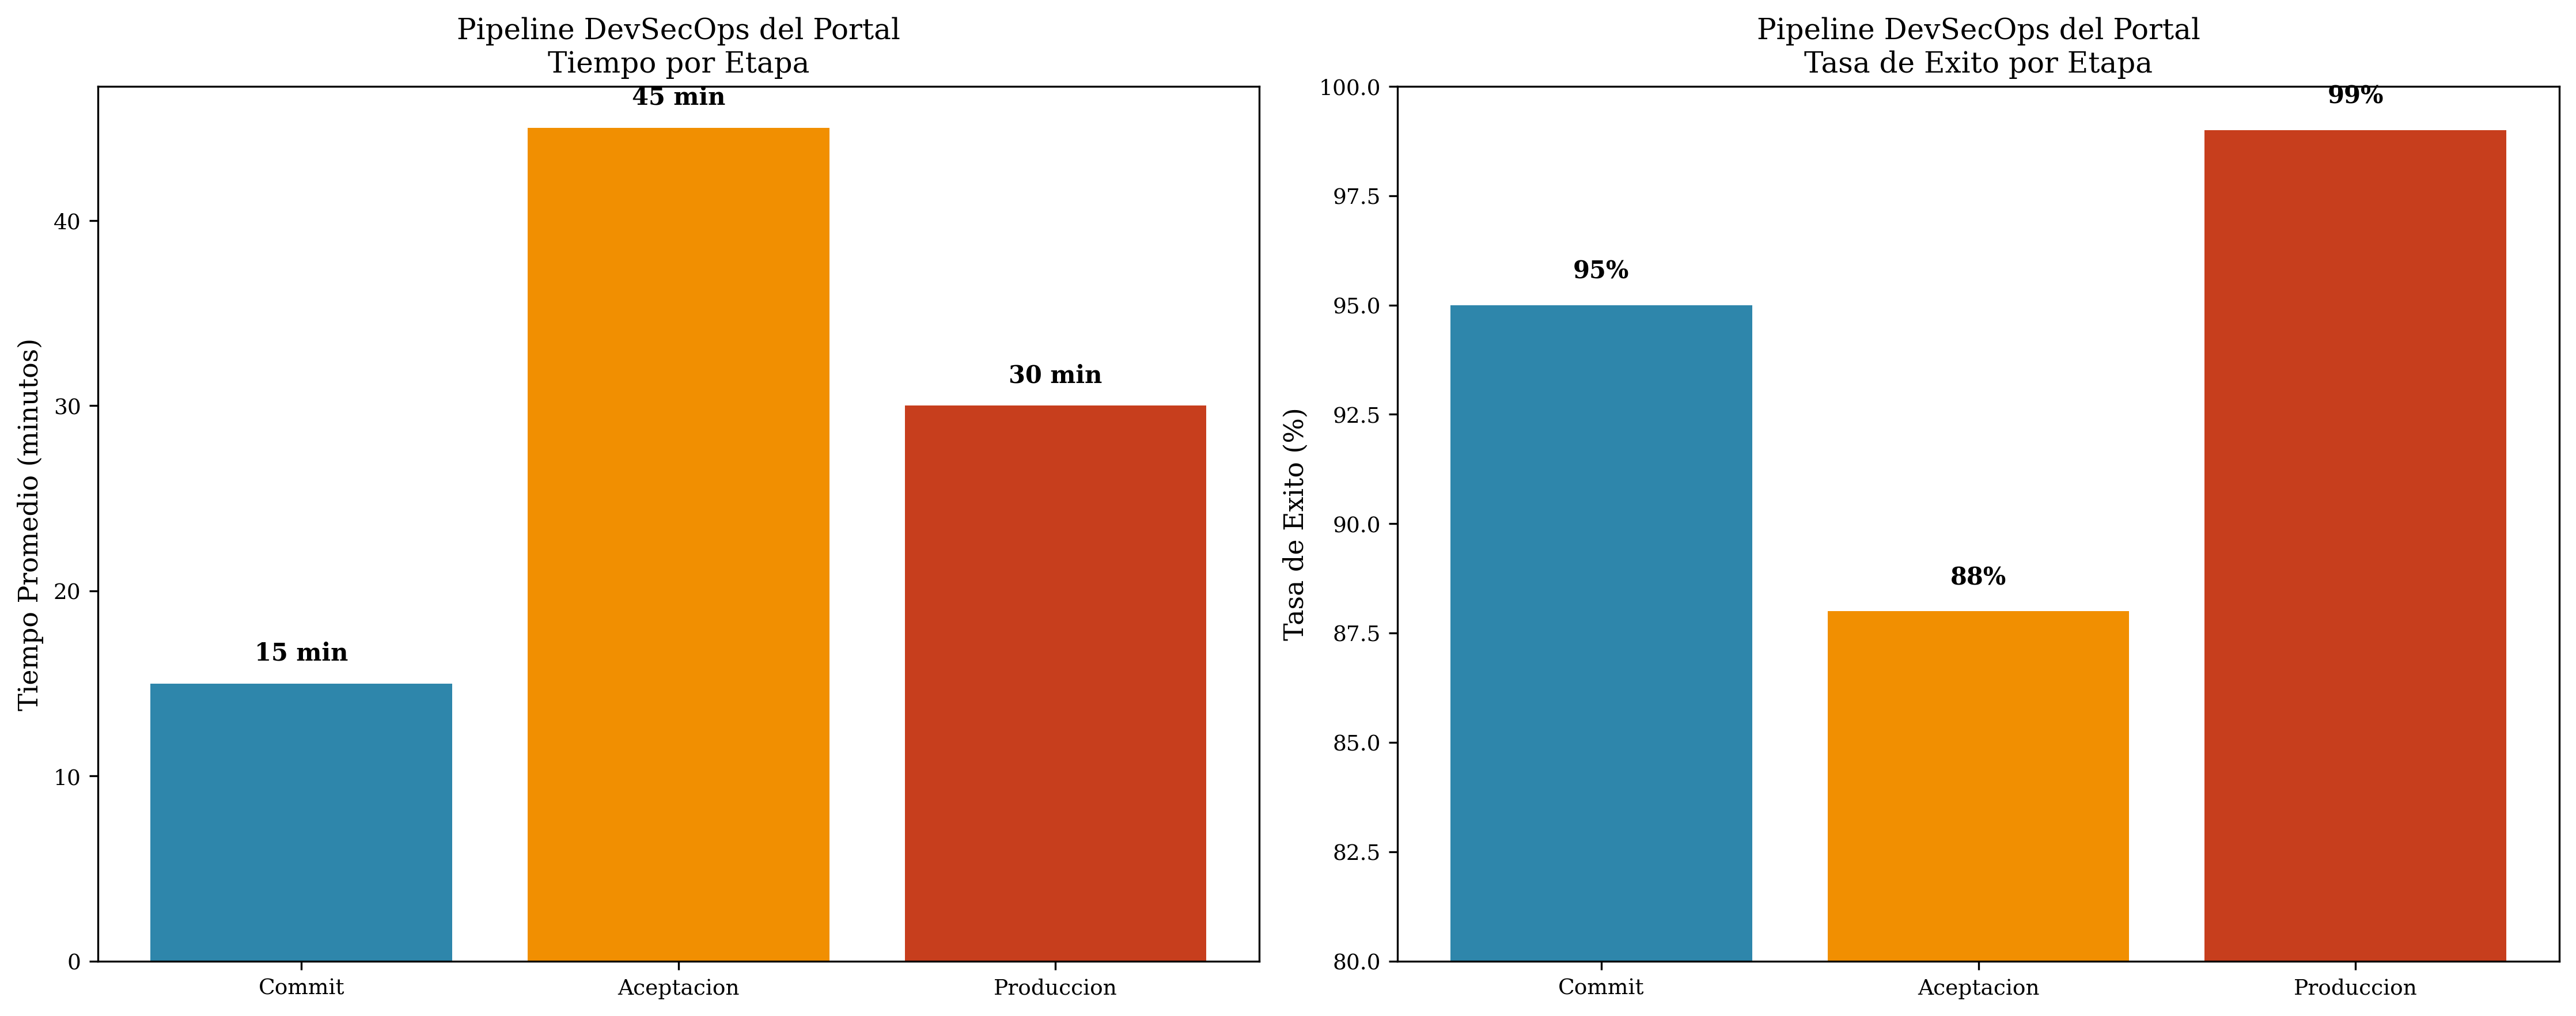
\includegraphics[width=0.45\textwidth]{graphics/pipeline_devsecops.png}
    \caption{Arquitectura completa del Pipeline DevSecOps y CI/CD}
    \label{fig:pipeline-devsecops-png}
\end{figure}

\begin{figure}[htbp]
    \centering
    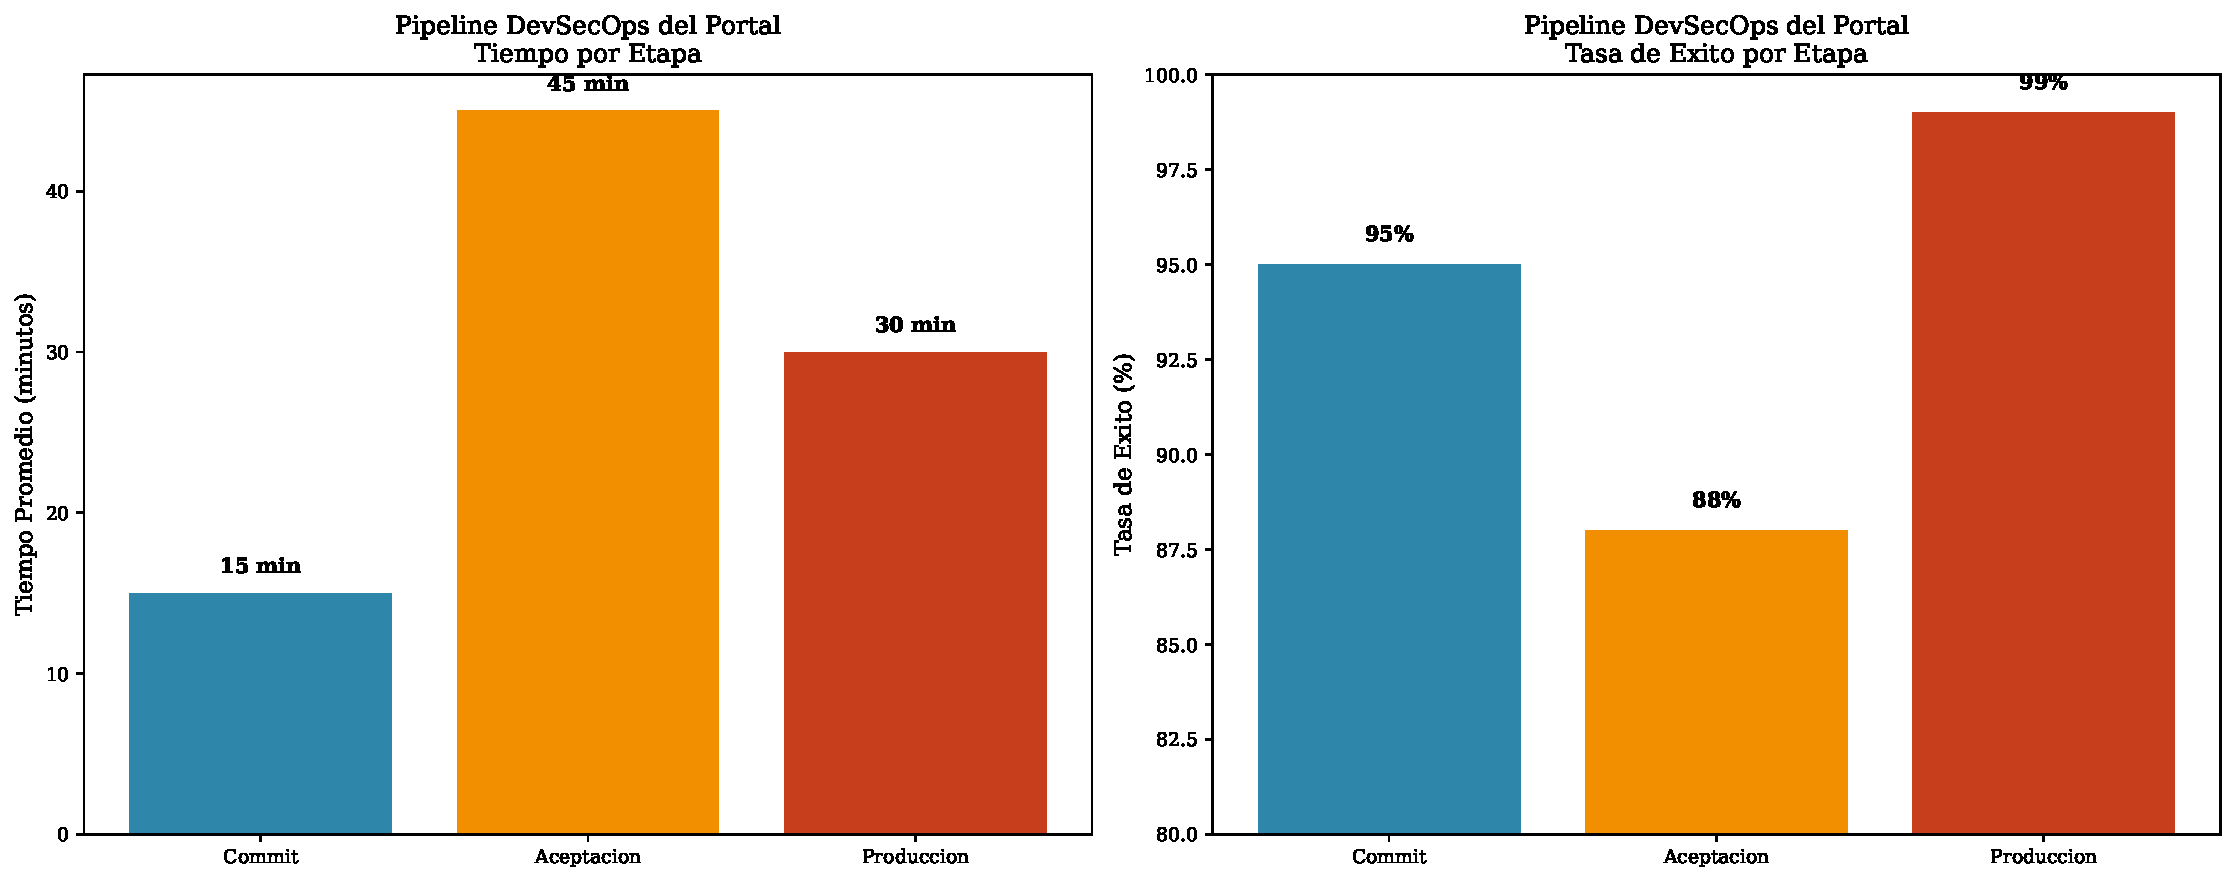
\includegraphics[width=0.48\textwidth]{graphics/pipeline_devsecops.pdf}
    \caption{Pipeline DevSecOps implementado en el Portal Agro-comercial del Huila}
    \label{fig:pipeline_devsecops}
\end{figure}